\documentclass[11pt,a4paper]{article}

\usepackage[T1]{fontenc}
\usepackage{lmodern}
\usepackage[margin=2.6cm]{geometry}
\usepackage{amsmath,amssymb,amsthm,mathtools}
\usepackage{booktabs,longtable,array}
\usepackage{tikz}
\usetikzlibrary{arrows.meta}
\usepackage[colorlinks=true,linkcolor=black,citecolor=black,urlcolor=black]{hyperref}
\usepackage{microtype}
\emergencystretch=1.5em

% ---------- Notation ----------
\newcommand{\R}{\mathbb{R}}
\newcommand{\N}{\mathbb{N}}
\newcommand{\ennr}{\ensuremath{[0,\infty]}}          % extended nonnegative reals
\newcommand{\vol}{\operatorname{vol}}                % Lebesgue measure / volume
\newcommand{\dd}{\mathrm{d}}
\DeclareMathOperator{\ediam}{ediam}
\DeclareMathOperator{\dist}{dist}
\DeclareMathOperator{\Hdim}{dim_H}
\newcommand{\HM}[1]{\mathcal{H}^{#1}}                % Hausdorff measure
\newcommand{\Plane}{\ensuremath{\mathbb{R}^{2}}}     % Euclidean plane
\newcommand{\FinTwo}{\ensuremath{\mathrm{Fin}\,2 \to \R}}
\newcommand{\dir}{\mathbf{u}}                        % unit direction vector
\newcommand{\tseg}{\sigma}                           % segment
\newcommand{\tube}{T}                                % tube
\newcommand{\ind}{\mathbf{1}}
\newcommand{\lname}[1]{\texttt{#1}}                  % Lean declaration names
\newcommand{\lb}{\_\allowbreak}                      % breakable underscore (long Lean names)

\newtheorem{theorem}{Theorem}[section]
\newtheorem{lemma}[theorem]{Lemma}
\newtheorem{proposition}[theorem]{Proposition}
\newtheorem{corollary}[theorem]{Corollary}
\theoremstyle{definition}
\newtheorem{definition}[theorem]{Definition}
\theoremstyle{remark}
\newtheorem{remark}[theorem]{Remark}

\title{The planar Kakeya theorem\\[2pt] \large A Lean~4 / Mathlib formalization}
\author{\texttt{Kakeya} Lean development\\[2pt]
  \small Lean 4.33.1 (\texttt{leanprover/lean4:v4.33.1}) with Mathlib}
\date{October 2026}

\begin{document}

\maketitle

\begin{abstract}
\noindent
This document describes a formalization, in Lean~4 with Mathlib, of the planar Kakeya
conjecture: every set in the plane that contains a translate of a unit segment in every
direction has Hausdorff dimension~$2$ (Davies, 1971).  The proof formalized here follows
C\'ordoba's $L^2$ route: a discrete operator (Schur) bound for thin tubes, a row-sum estimate
of order $h^{2}N(1+\log N)$, and a multi-scale covering argument converting the operator
bound into a lower bound for the $d$-dimensional diameter sum of \emph{every} countable
cover of the set, for every $d<2$.  We present the architecture of the development, the
formal statements of all key definitions and lemmas together with their mathematical
meaning, proof outlines that follow the formal proofs, and a declaration-by-declaration
correspondence table.  All statements below are reproduced faithfully from the Lean
sources; the main theorem carries no hypotheses beyond the Kakeya property, and the only
axioms used are Lean's three standard ones.
\end{abstract}

\tableofcontents

%=====================================================================
\section{Introduction}
%=====================================================================

A \emph{Kakeya set} (or \emph{Besicovitch set}) in the plane is a set $E\subseteq\Plane$
that contains a translate of the unit segment in every direction.  Besicovitch showed that
such sets can have Lebesgue measure zero \cite{Besicovitch1928}, and the \emph{Kakeya
conjecture in dimension two} asserts that they nevertheless have full Hausdorff dimension:

\begin{theorem}[Planar Kakeya theorem; {\lname{Kakeya.planar\_kakeya\_hausdorff\_dimension}}]
\label{thm:main}
Let $E\subseteq\Plane$ be a Kakeya set.  Then $\Hdim E = 2$.
\end{theorem}

The theorem was first proved by Davies \cite{Davies1971} via pole/polar duality, Marstrand's
projection theorem and the product (slicing) theorem for Hausdorff measures.  The
formalization described here takes instead the route of C\'ordoba \cite{Cordoba1977}, which
requires only elementary tube geometry, a discrete $L^2$ (operator) bound, and a
multi-scale covering argument organized over dyadic scales; this route is better matched to
what is available in Mathlib today.  The two models of the plane used in the development ---
the Euclidean plane $\Plane$ (\lname{EuclideanSpace}~$\R$~\lname{(Fin 2)}) and the sup-norm model
$\FinTwo$ --- are related by a linear map of Lipschitz constant $1$ and anti-Lipschitz
constant $\sqrt{2}$, so Hausdorff dimension transfers between them freely.

\subsection{What is formalized}

The development consists of $14$ Lean modules, about $2800$ lines, in the namespace
\lname{Kakeya}.  The main statement is

\begin{center}
\lname{theorem planar\_kakeya\_hausdorff\_dimension (E : Set Plane)
        (hE : IsKakeyaSet E) : dimH E = 2}
\end{center}

\noindent
where \lname{dimH} is Mathlib's Hausdorff dimension with values in $\ennr$.  The statement
is unconditional: no boundedness, measurability or Borel hypotheses, and no \lname{sorry}.
Checking the kernel axioms of the final theorem yields only \lname{propext},
\lname{Classical.choice} and \lname{Quot.sound}; in particular there is no
\lname{sorryAx}.  The hypothesis \lname{IsKakeyaSet E} is genuinely restrictive (a
singleton is not a Kakeya set), and the conclusion is non-trivial (a singleton has
dimension $0$).

\subsection{Overview of the argument}

The heart of the proof is the following quantitative statement: for every exponent $d<2$
there is a constant $c(d)>0$ such that \emph{every} countable cover
$(t_n)_{n\in\N}$ of a Kakeya set $E$, by sets of diameter at most $1/16$, satisfies
\begin{equation}\label{eq:coverbound}
  \sum_{n}\, (\ediam t_n)^{d}\ \ge\ c(d).
\end{equation}
This is \lname{cover\_sum\_bound} (Theorem~\ref{thm:cover-sum-bound}).  Since the
$d$-dimensional Hausdorff measure is defined as a supremum over infima of exactly such
sums, \eqref{eq:coverbound} implies $\HM{d}(E)\neq 0$ for all $d<2$, hence
$\Hdim E \ge 2$; the matching upper bound $\Hdim E\le 2$ holds for every subset of the
plane.  The covering bound itself is proved in four moves:

\begin{enumerate}
\item \textbf{Desertification into scales.}  The cover is split into dyadic layers
  $J_k = \{n : 2^{-(k+1)}<\ediam t_n\le 2^{-k}\}$, refined into pairwise disjoint
  measurable sets $H_k$ with $\bigcup_k H_k = \bigcup_k G_k$,
  $G_k=\bigcup_{n\in J_k}\overline{t_n}$.
\item \textbf{One-dimensional coverage.}  Along each Kakeya segment of direction $\theta$,
  the layers cover a set of parameters of total length at least $3/4$:
  $\sum_k \lambda(k,\theta)\ge 3/4$, where $\lambda(k,\theta)$ is the measure of the
  parameters in $[-3/8,3/8]$ landing in $H_k$.
\item \textbf{Tube estimate.}  A thickened piece of the segment lies in any tube whose
  direction is within $4\cdot 2^{-k}$ of $\theta$, so the coverage converts into
  $|T\cap F_k|\ge c_k\,\delta_k$ for the tubes $T$ of direction $\pi i/2^k$, where
  $F_k$ is a neighbourhood of $G_k$ and $\delta_k=2^{-k}$; an area lemma
  (a rotated box of volume $2r|A|$ inside a thickening) supplies the factor.
\item \textbf{Operator bound and pigeonhole.}  A discrete second-moment estimate
  ($\sum_i |T_i\cap S|^2\le 2M|S|$), fed with a row-sum bound
  $M\asymp k\,2^{-k}$ coming from the two-tube intersection estimate, together with a
  weighted pigeonhole over the $2^k$ direction arcs, produces enough ``good'' tubes at
  each scale to make the weighted sum over scales at least $1$, and assembling scale by
  scale gives \eqref{eq:coverbound} with the explicit constant
  $c(d)=\delta(d)^{2}\,2^{-d}/130000$.
\end{enumerate}

%=====================================================================
\section{Modules and dependencies}
%=====================================================================

The development is organised in three layers.

\begin{description}
\item[Layer A (analytic and discrete inputs).]  Elementary estimates: the harmonic sum
  bound, trigonometric lower bounds for $\sin(\pi m/N)$, the Schur test, and the abstract
  second-moment (Cauchy--Schwarz) inequality for a finite family of measurable sets.
\item[Layer B (geometry and the operator bound).]  Rotations, rectangles, tubes and strips
  in $\FinTwo$; the two-tube intersection bound; the row-sum estimate for the matrix of
  pairwise tube intersections; the discrete Kakeya operator bound.
\item[Layer C (from tubes to Hausdorff dimension).]  The multi-scale covering argument,
  the conversion of covering bounds into Hausdorff-measure nonvanishing, the transfer
  between the two models of the plane, and the main theorem.
\end{description}

\begin{figure}[ht]
\centering
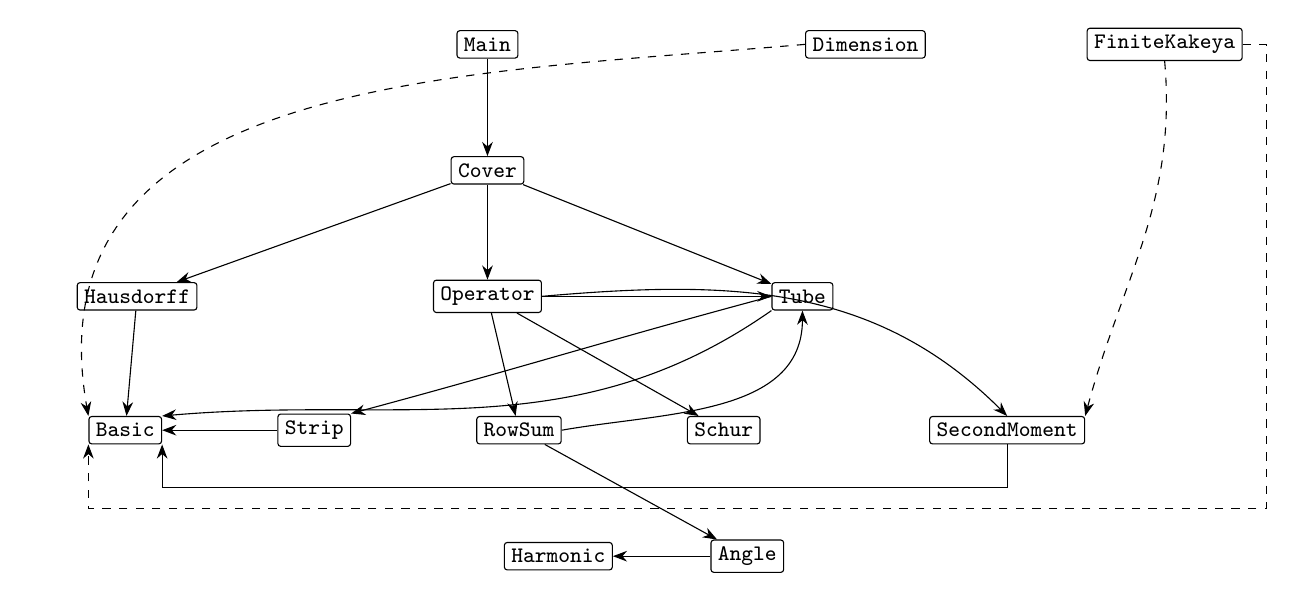
\begin{tikzpicture}[
  font=\footnotesize\ttfamily,
  every node/.style={draw, rounded corners=1pt, inner sep=2.5pt, fill=white},
  side/.style={dashed},
  ar/.style={-{Stealth[length=1.8mm]}, thin}]

  \node (Main) at (0,0) {Main};
  \node (Dimension) at (4.8,0) {Dimension};
  \node (FiniteKakeya) at (8.6,0) {FiniteKakeya};

  \node (Cover) at (0,-1.6) {Cover};
  \node (Hausdorff) at (-4.45,-3.2) {Hausdorff};
  \node (Operator) at (0,-3.2) {Operator};
  \node (Tube) at (4.0,-3.2) {Tube};

  \node (Basic) at (-4.6,-4.9) {Basic};
  \node (Strip) at (-2.2,-4.9) {Strip};
  \node (RowSum) at (0.4,-4.9) {RowSum};
  \node (Schur) at (3.0,-4.9) {Schur};
  \node (SecondMoment) at (6.6,-4.9) {SecondMoment};

  \node (Harmonic) at (0.9,-6.5) {Harmonic};
  \node (Angle) at (3.3,-6.5) {Angle};

  \draw[ar] (Main) -- (Cover);
  \draw[ar] (Cover) -- (Hausdorff);
  \draw[ar] (Cover) -- (Operator);
  \draw[ar] (Cover) -- (Tube);
  \draw[ar] (Operator) -- (Tube);
  \draw[ar] (Operator) -- (Schur);
  \draw[ar] (Operator) -- (RowSum);
  \draw[ar] (Operator.east) to[out=5,in=135] (SecondMoment.north);
  \draw[ar] (RowSum) -- (Angle);
  \draw[ar] (RowSum.east) to[out=10,in=270] (Tube.south);
  \draw[ar] (Tube.west) to[out=195,in=15] (Strip.north east);
  \draw[ar] (Tube.south west) to[out=215,in=5] (Basic.north east);
  \draw[ar] (Strip) -- (Basic);
  \draw[ar] (Angle) -- (Harmonic);
  \draw[ar] (Hausdorff) -- (Basic);
  \draw[ar] (SecondMoment.south) -- ++(0,-0.55) -| (Basic.south east);
  \draw[ar, side] (Dimension.west) to[out=185,in=100,looseness=1.1] (Basic.north west);
  \draw[ar, side] (FiniteKakeya.south) to[out=275,in=75] (SecondMoment.north east);
  \draw[ar, side] (FiniteKakeya.east) -- ++(0.3,0) -- ++(0,-5.9) -| (Basic.south west);

\end{tikzpicture}
\caption{Module import structure.  \texttt{Main} imports only \texttt{Cover}; the modules
\texttt{Dimension} (the upper bound on $\Hdim$ in the \lname{Plane} model) and
\texttt{FiniteKakeya} (the standalone finite Kakeya estimate, Layer~B) are shown dashed:
they are part of the development but not in \texttt{Main}'s import cone --- the working
upper bound is \lname{dimH\lb le\lb two\lb fin2} in \texttt{Hausdorff.lean}.}
\label{fig:modules}
\end{figure}

Table~\ref{tab:modules} lists the modules with their roles; the full declaration-level
correspondence is in Section~\ref{sec:correspondence}.

\begin{table}[ht]
\centering\small
\begin{tabular}{@{}ll@{}}
\toprule
Module & Contents \\
\midrule
\lname{Basic.lean}        & plane model, directions, segments, Kakeya sets, thin tubes \\
\lname{Harmonic.lean}     & $\sum_{d=1}^{N}1/d\le 1+\log N$; $\sin(\pi d/N)\ge 2d/N$ \\
\lname{Angle.lean}        & $|\sin(\pi m/N)|\ge 2\min(|m|,N-|m|)/N$, nonvanishing of sines \\
\lname{Strip.lean}        & horizontal/angled strips; the two-strip area estimate \\
\lname{Tube.lean}         & rotations, rectangles, tubes, measurability, two-tube bound \\
\lname{SecondMoment.lean} & $(\sum_i\mu T_i)^2\le(\sum_{i,j}\mu(T_i\cap T_j))\cdot\mu(\bigcup_i T_i)$ \\
\lname{Schur.lean}        & the symmetric Schur test (real version) \\
\lname{RowSum.lean}       & harmonic reindexings; row sums $\le 2h+20h^2N(1+\log N)$ \\
\lname{Operator.lean}     & Schur test in $\ennr$; $\sum_i\mu(T_i\cap S)^2\le 2M\,\mu S$ \\
\lname{FiniteKakeya.lean} & the finite estimate $Nc^2\le M\,\mu(\bigcup_i T_i)$ \\
\lname{Hausdorff.lean}    & cover bound $\Rightarrow \HM{d}\ne 0 \Rightarrow \Hdim\ge 2$; model transfer \\
\lname{Cover.lean}        & the multi-scale covering bound (the heart) \\
\lname{Dimension.lean}    & $\Hdim E\le 2$ for $E\subseteq\Plane$ \\
\lname{Main.lean}         & the final theorem $\Hdim E = 2$ \\
\bottomrule
\end{tabular}
\caption{The 14 modules of the \lname{Kakeya} development ($\approx 2813$ lines of Lean).}
\label{tab:modules}
\end{table}

%=====================================================================
\section{Basic notions (\lname{Basic.lean}, \lname{Hausdorff.lean})}
%=====================================================================

\subsection{Two models of the plane}

The statements live in the Euclidean plane, while the quantitative tube computations are
done in the sup-norm model, where boxes are easy to handle.

\begin{definition}[{The plane; \lname{Kakeya.Plane}}] $\Plane$ is
\lname{EuclideanSpace}~$\R$~\lname{(Fin 2)}, i.e.\ $\R^2$ with the Euclidean norm,
realized as \lname{WithLp}~$2$~$(\FinTwo)$.  The \emph{sup-norm model} \FinTwo{} carries
the product
structure; \lname{WithLp.ofLp} identifies the two.
\end{definition}

\begin{definition}[{Directions; \lname{Kakeya.dir}, \lname{Kakeya.dirFi2}}]
For $\theta\in\R$, $\dir(\theta) = (\cos\theta,\sin\theta)$, as an element of $\Plane$
(\lname{dir}) resp.\ $\FinTwo$ (\lname{dirFi2}).
\end{definition}

\begin{lemma}[{unit vectors and frames; \lname{norm\_dir}, \lname{inner\_dir},
\lname{inner\lb dir\lb perp}, \lname{eq\lb inner\lb decomp}}]\  \label{lem:frame}
\begin{enumerate}
\item $\|\dir(\theta)\|=1$.
\item $\langle \dir(\theta),\dir(\phi)\rangle = \cos(\theta-\phi)$; in particular
$\langle \dir(\theta),\dir(\theta+\pi/2)\rangle=0$.
\item Every $x\in\Plane$ expands in the orthonormal frame
$(\dir(\theta),\dir(\theta+\pi/2))$:
\[
  \langle x,\dir(\theta)\rangle\cdot\dir(\theta)
  + \langle x,\dir(\theta+\pi/2)\rangle\cdot\dir(\theta+\pi/2) = x .
\]
\end{enumerate}
\end{lemma}

\begin{definition}[{segments, Kakeya sets; \lname{cseg}, \lname{seg}, \lname{IsKakeyaSet}}]
The \emph{unit segment of direction $\theta$ centred at $a$} is
\[
  \tseg(\theta,a) \;=\; \{\, a + t\,\dir(\theta) : t\in[-\tfrac12,\tfrac12] \,\}
\]
(written \lname{cseg} in $\Plane$ and \lname{seg} in $\FinTwo$).  A set
$E\subseteq\Plane$ is a \emph{Kakeya set},
\lname{IsKakeyaSet E}, if $\forall\theta,\ \exists\,a,\ \tseg(\theta,a)\subseteq E$.
\end{definition}

\begin{definition}[{thin tubes; \lname{planeTube}, \lname{tube}, \lname{rect}}]
The \emph{tube of length $1$, width $2h$, direction $\theta$, centre $a$} is
\[
  \tube_{h,\theta}(a)
  = \{\, x : |\langle x-a,\dir(\theta)\rangle|\le \tfrac12,\;
             |\langle x-a,\dir(\theta+\pi/2)\rangle|\le h \,\}.
\]
In the sup-norm model it is the preimage under the rigid motion
$p\mapsto R_\theta(p-a)$ of the \emph{standard rectangle}
$\lname{rect}(h) = [-1/2,1/2]\times[-h,h]$, where $R_\theta$
(\lname{rotLin}) is the (clockwise) rotation by $\theta$, given by the matrix
$\begin{psmallmatrix}\cos\theta & \sin\theta\\ -\sin\theta & \cos\theta\end{psmallmatrix}$
(\lname{rotM}).
\end{definition}

\begin{lemma}[{tubes thicken their axes; \lname{planeTube\_subset\_cthickening}}]
\label{lem:tube-thicken}
$\tube_{h,\theta}(a)$ is contained in the closed $h$-neighbourhood of $\tseg(\theta,a)$.
Hence every Kakeya set has, in every direction $\theta$, a whole tube inside its closed
$h$-neighbourhood
(\lname{IsKakeyaSet.exists\lb planeTube\lb subset\lb cthickening}).
\end{lemma}

\begin{remark}
All quantitative work below (strips, tubes, the covering argument) takes place in the
sup-norm model $\FinTwo$; Section~\ref{sec:transfer} explains the transfer back to
$\Plane$.
\end{remark}

%=====================================================================
\section{Elementary analytic inputs (\lname{Harmonic.lean}, \lname{Angle.lean})}
%=====================================================================

\begin{lemma}[{harmonic sum bound; \lname{sum\_Icc\_inv\_le\_one\_add\_log}}]
For every $N\in\N$,
\[
  \sum_{d=1}^{N} \frac{1}{d} \;\le\; 1 + \log N .
\]
\emph{In Lean this is the cast of Mathlib's \lname{harmonic\_le\_one\_add\_log}.}
\end{lemma}

\begin{lemma}[{sine lower bounds; \lname{sin\lb pi\lb mul\lb div\lb lower},
\lname{abs\lb sin\lb pi\lb div\lb lower}, \lname{sin\lb abs\lb lower}}]\ 
\begin{enumerate}
\item If $2d\le N$ then $\sin(\pi d/N)\ge \dfrac{2d}{N}$.
\item If $0\le x\le N$ then $\sin(\pi x/N)\ge \dfrac{2\min(x,\,N-x)}{N}$.
\item If $|m|\le N$ then
$\bigl|\sin(\pi m/N)\bigr|\ge \dfrac{2\min(|m|,\,N-|m|)}{N}$.
\end{enumerate}
\emph{These follow from the concavity estimate $\sin u\ge \tfrac{2}{\pi}u$ on
$[0,\pi/2]$ (Mathlib's \lname{Real.mul\_le\_sin}) and the symmetry
$\sin(\pi - u)=\sin u$.}
\end{lemma}

\begin{lemma}[{distinct directions are angularly separated;
\lname{sin\_pi\_div\_fin\_ne}}]
For distinct $i,j\in\{0,\dots,N-1\}$, $\sin\bigl(\pi(j-i)/N\bigr)\neq 0$.
\end{lemma}

\begin{lemma}[{\lname{inv\_min\_le}}] For $a,b>0$,
$(\min(a,b))^{-1}\le a^{-1}+b^{-1}$.
\end{lemma}

%=====================================================================
\section{Discrete $L^2$ machinery}
%=====================================================================

\emph{Modules: \lname{SecondMoment.lean}, \lname{Schur.lean}, \lname{FiniteKakeya.lean},
\lname{Operator.lean}.}

\medskip
All measure-theoretic quantities in this section are extended nonnegative reals,
$\mu(\,\cdot\,)\in\ennr$.

\begin{theorem}[{second-moment inequality; \lname{second\_moment}}]
\label{thm:second-moment}
Let $(\alpha,\mu)$ be a measure space, $\iota$ a finite index set, and
$T_i\subseteq\alpha$ measurable.  Then
\[
  \Bigl(\sum_i \mu(T_i)\Bigr)^{2}
    \;\le\; \Bigl(\sum_{i}\sum_{j} \mu(T_i\cap T_j)\Bigr)\cdot
             \mu\Bigl(\bigcup_i T_i\Bigr).
\]
\end{theorem}

\begin{proof}[Proof outline (as formalized)]
Set $s=\bigcup_i T_i$ and $g=\sum_i \ind_{T_i}$.  Then
$\int g\,\dd\mu = \sum_i \mu(T_i)$ and --- expanding the square indicatorwise ---
$\int g^2\,\dd\mu = \sum_{i,j}\mu(T_i\cap T_j)$.  Since $g=0$ off $s$,
$g = g\,\ind_s$, and H\"older's inequality
$\int g\,\ind_s \le \|g\|_2\,\|\ind_s\|_2$
(Mathlib's \lname{ENNReal.lintegral\_mul\_le\_Lp\_mul\_Lq} at $p=q=2$) gives
$(\sum_i\mu T_i)^2 \le (\int g^2)\,\mu(s)$.  Squaring in $\ennr$ is undone by
\lname{rpow\_half\_mul\_self}.
\end{proof}

\begin{theorem}[{finite Kakeya bound; \lname{finite\_kakeya\_bound},
\lname{finite\_kakeya\_bound\_div}}]
If $Nc\le \sum_i\mu(T_i)$ and $\sum_{i,j}\mu(T_i\cap T_j)\le M$, then
$(Nc)^2\le M\cdot\mu(\bigcup_i T_i)$; when $M$ is finite and nonzero,
$\mu(\bigcup_i T_i)\ge (Nc)^2/M$.
\end{theorem}

\begin{remark}
With $N\approx 1/\delta$ tubes of area $c=2\delta$ and pairwise-overlap total
$M\lesssim \log(1/\delta)$ this is C\'ordoba's bound
$|\bigcup_i T_i|\gtrsim 1/\log(1/\delta)$.  In the present development the finite
estimate is not on the dependency path of the main theorem: the multi-scale argument of
Section~\ref{sec:cover} uses the operator form below instead.
\end{remark}

\begin{theorem}[{symmetric Schur test; \lname{schur\_test} (real form),
\lname{schur\_test\_ennreal} ($\ennr$ form)}]
Let $B=(B_{ij})$ be symmetric with $B_{ij}\ge 0$ and all row sums at most $M$.  Then
\[
  \sum_{i,j} c_i c_j B_{ij} \;\le\; M \sum_i c_i^{2}
  \qquad\text{(\,$\le 2M\sum_i c_i^2$ in the $\ennr$ form).}
\]
\end{theorem}

\begin{proof}[Proof outline]
From $c_ic_j \le |c_i||c_j| \le \tfrac12(c_i^2+c_j^2)$
(in $\ennr$: $c_ic_j\le c_i^2+c_j^2$, \lname{ENNReal.mul\lb le\lb add\lb sq}), split the double
sum into a ``row'' part $\sum_i c_i^2\sum_j B_{ij}$ and a ``column'' part
$\sum_j c_j^2\sum_i B_{ij}$ (reindexed by symmetry), and bound each by $M\sum_i c_i^2$.
\end{proof}

\begin{theorem}[{operator bound, abstract form; \lname{operator\_bound\_general}}]
\label{thm:operator-bound-general}
Let $T_i$ be measurable, $S$ measurable, and suppose every row sum of the pairwise
intersection masses is at most $M$: $\sum_j \mu(T_i\cap T_j)\le M$ for all $i$.  Then
\[
  \sum_i \mu(T_i\cap S)^{2}\;\le\; 2M\,\mu(S).
\]
\end{theorem}

\begin{proof}[Proof outline (as formalized)]
Let $w_i=\mu(T_i\cap S)$ and $F=\sum_i w_i\ind_{T_i}$.  Two pointwise identities,
checked indicator by indicator, give
\[
  \int_S F\,\dd\mu = \sum_i w_i^2,
  \qquad
  \int F^{2}\,\dd\mu = \sum_{i,j} w_i w_j\,\mu(T_i\cap T_j).
\]
The Schur test with $B_{ij}=\mu(T_i\cap T_j)$ bounds the right-hand side by
$2M\sum_i w_i^2$.  H\"older's inequality applied to $F\cdot\ind_S$ gives
$\sum_i w_i^2 \le (\int F^2)^{1/2}\mu(S)^{1/2}$; substituting and squaring yields
$(\sum_i w_i^2)^2\le 2M(\sum_i w_i^2)\,\mu(S)$, and cancelling the finite nonzero factor
(cases $\sum_i w_i^2=0$, $M=\infty$ handled separately) gives the claim.
\end{proof}

%=====================================================================
\section{Tube geometry (\lname{Strip.lean}, \lname{Tube.lean}, \lname{RowSum.lean})}
%=====================================================================

Throughout, $\vol$ is Lebesgue measure on $\FinTwo\simeq\R^2$ (with the sup norm, so the
product-box formula $\vol([a,b])=\prod_i(b_i-a_i)$ applies), and
$h>0$.

\begin{lemma}[{rigid motions preserve area; \lname{det\_rotLin}, \lname{volume\_rotLin},
\lname{volume\_image\_add}}]
$\det R_\theta = 1$, hence $\vol(R_\theta A)=\vol(A)$; translations preserve volume too.
\end{lemma}

\begin{lemma}[{area of a tube; \lname{volume\_rect}, \lname{volume\_tube}}]
$\vol(\lname{rect}(h)) = 2h$ and $\vol(\tube_{h,\theta}(a))=2h$; tubes are measurable
(\lname{measurableSet\_tube}).
\end{lemma}

\begin{definition}[{strips; \lname{hstrip}, \lname{astrip}}]
$\lname{hstrip}(h,t)=\{p : |p_1 - t|\le h\}$ is a horizontal strip of half-width $h$;
$\lname{astrip}(a,b,h,u)=\{p : |a p_0 + b p_1 - u|\le h\}$ is the strip with normal
$(a,b)$ of half-width $h$.
\end{definition}

\begin{lemma}[{two-strip estimate; \lname{volume\_hstrip\_inter\_astrip}}]
\label{lem:two-strip}
For $a\neq0$ and $h\ge0$,
\[
  \vol(\lname{hstrip}(h,t)\cap \lname{astrip}(a,b,h,u))
  \;\le\; 2\,\frac{h+|b|\,h}{|a|}\cdot(2h).
\]
\end{lemma}

\begin{proof}[Proof outline]
The triangle inequality $|a p_0-(u-bt)|\le |a p_0 + b p_1 - u| + |b|\,|p_1 - t|
\le h+|b|h$ shows the intersection is contained in the axis-parallel box
$[(u-bt\pm(h+|b|h))/a]\times[t-h,t+h]$, of area exactly the right-hand side; the case
$a>0$ (\lname{volume\_hstrip\_inter\_astrip\_pos}) extends to $a\ne0$ by
\lname{astrip\_neg}.
\end{proof}

\begin{theorem}[{two-tube intersection bound; \lname{volume\_tube\_inter\_le}}]
\label{thm:two-tube}
Let $\psi=\phi-\theta$ with $\sin\psi\neq0$.  For any centres $a,b$,
\[
  \vol\bigl(\tube_{h,\theta}(a)\cap \tube_{h,\phi}(b)\bigr)
  \;\le\; 2\,\frac{h+|\cos\psi|\,h}{|\sin\psi|}\cdot(2h)
  \;=\; \frac{4h^2(1+|\cos\psi|)}{|\sin\psi|}.
\]
\end{theorem}

\begin{proof}[Proof outline]
Rotating the whole configuration by $\theta$ (which preserves area) makes the first tube
lie in a horizontal strip; the second tube then lies in an angled strip with normal
$(-\sin\psi,\cos\psi)$ (Lemmas \lname{tube\_subset\_astrip},
\lname{tube\_inter\_subset}, using $R_\alpha\circ R_\beta = R_{\alpha+\beta}$,
\lname{rotLin\_comp}).  Apply the two-strip estimate with $|a|=|\sin\psi|$,
$|b|=|\cos\psi|$.
\end{proof}

\begin{lemma}[{intersections of regularly spaced tubes; \lname{tube\_inter\_toReal\_le}}]
\label{lem:tube-inter-real}
Let $N\ge1$, and for $i\in\{0,\dots,N-1\}$ put $\theta_i=\pi i/N$.  For $i\neq j$ and any
centres $a,b$,
\[
  \vol\bigl(\tube_{h,\theta_i}(a)\cap \tube_{h,\theta_j}(b)\bigr)
  \;\le\; 4h^2 N\Bigl(\frac{1}{|j-i|}+\frac{1}{N-|j-i|}\Bigr).
\]
\end{lemma}

\begin{proof}[Proof outline]
Combine Theorem~\ref{thm:two-tube} (with $1+|\cos|\le 2$) with
$|\sin(\pi m/N)|\ge 2\min(|m|,N-|m|)/N$ for $m=j-i$
(\lname{sin\_abs\_lower}, the angle difference being nonzero by
\lname{sin\lb pi\lb div\lb fin\lb ne}), and \lname{inv\lb min\lb le}.
\end{proof}

\begin{theorem}[{row-sum bound; \lname{row\_sum\_le}}]
\label{thm:row-sum}
For $N$ equally spaced directions $\theta_i=\pi i/N$, any centre assignment
$a_i$, and any fixed row $i$,
\[
  \sum_{j=0}^{N-1} \vol\bigl(\tube_{h,\theta_i}(a_i)\cap \tube_{h,\theta_j}(a_j)\bigr)
  \;\le\; 2h + 20\,h^{2}N\,(1+\log N).
\]
\end{theorem}

\begin{proof}[Proof outline]
The diagonal term is $\vol(\tube)=2h$.  For the off-diagonal sum,
Lemma~\ref{lem:tube-inter-real} leaves the two distance sums
$\sum_{j\ne i} 1/|j-i|\le 2\sum_{k=1}^N 1/k$ and
$\sum_{j\ne i} 1/(N-|j-i|)\le 3\sum_{k=1}^N 1/k$; the reindexing lemmas
(\lname{sum\_fin\_dist\_le}, \lname{sum\_inv\_abs\_sub\_le},
\lname{sum\_inv\_sub\_abs\_sub\_le}) bound a distance sum over $\mathrm{Fin}\,N$ by $f(0)$
plus two or three times the harmonic sum, and
$\sum_{k=1}^N 1/k\le 1+\log N$ closes the estimate:
the off-diagonal total is at most $4h^2N\cdot 5(1+\log N)$.
\end{proof}

\begin{theorem}[{discrete Kakeya operator bound; \lname{operator\_bound}}]
\label{thm:operator-bound}
For $N$ equally spaced directions, tubes of width $2h$, and any measurable set
$S\subseteq\FinTwo$,
\[
  \sum_{i=0}^{N-1} \vol\bigl(\tube_{h,\theta_i}(a_i)\cap S\bigr)^{2}
  \;\le\; 2\bigl(2h+20h^2N(1+\log N)\bigr)\cdot \vol(S).
\]
\end{theorem}

\begin{proof}
Instantiate Theorem~\ref{thm:operator-bound-general} with
$B_{ij}=\vol(T_i\cap T_j)$, whose row sums are at most
$R=2h+20h^2N(1+\log N)$ by Theorem~\ref{thm:row-sum} (each intersection has finite
measure, so $\ennr$ and real-valued sums agree).
\end{proof}

%=====================================================================
\section{The multi-scale covering argument (\lname{Cover.lean})}
\label{sec:cover}
%=====================================================================

This section is the heart of the formalization.  Fix a Kakeya set $E\subseteq\FinTwo$
(through the maps \lname{dirFi2}, \lname{seg}), an exponent $0<d<2$, and a countable
cover $E\subseteq\bigcup_n t_n$ with $\ediam t_n\le 1/16$ for all $n$.

\subsection{The scale decomposition}

\begin{definition}[{scales, layers, boxes, coverage function;
\lname{cover\_setup}}]\ \label{def:cover-setup}
\begin{itemize}
\item $u_n=\overline{t_n}$ (the closure, so $\ediam u_n=\ediam t_n$), and
$\rho_n = (\ediam u_n)_{\mathrm{toReal}}\ge 0$, which satisfies
$\ediam u_n = \rho_n$ (as an element of $\ennr$) and $\rho_n\le 1/16$.
\item $\delta_k = 2^{-k}$ and the \emph{scale layers}
\[
   J_k \;=\; \{\, n : \delta_{k+1}<\rho_n\le \delta_k \,\},
\]
pairwise disjoint, and empty for $k<4$ (since $\rho_n\le1/16=\delta_4$).
\item For nonempty $u_n$ pick $c_n\in u_n$ (by choice); the \emph{box}
$B_n=[c_n-\rho_n\mathbf{1},\,c_n+\rho_n\mathbf{1}]$ contains $u_n$ and satisfies
$\vol(B_n)\le (2\rho_n)^2$.
\item $G_k=\bigcup_{n\in J_k} u_n$ and the \emph{disjoint refinement}
$H_k = G_k\setminus\bigcup_{k'<k}G_{k'}$; the $H_k$ are measurable, pairwise disjoint,
empty for $k<4$, and $\bigcup_k H_k=\bigcup_k G_k$ (take the first layer containing a
point).
\item For each direction $\theta$, choose (by choice, from the Kakeya property) a centre
$a(\theta)$ with $\tseg(\theta,a(\theta))\subseteq E$; write
$\mathrm{par}_\theta(x)=a(\theta)+x\,\dir(\theta)$ and the \emph{coverage function}
\[
  \lambda(k,\theta)
  \;=\; \vol\bigl(\mathrm{par}_\theta^{-1}(H_k)\cap[-\tfrac38,\tfrac38]\bigr).
\]
\end{itemize}
\end{definition}

\begin{theorem}[{the covering setup; \lname{cover\_setup}}]
\label{thm:cover-setup}
With the data of Definition~\ref{def:cover-setup}, for every direction $\theta$,
\[
  \frac34 \;\le\; \sum_{k\in\N} \lambda(k,\theta) .
\]
\end{theorem}

\begin{proof}[Proof outline]
The image of $x\in[-3/8,3/8]$ under $\mathrm{par}_\theta$ lies in
$E\subseteq\bigcup_n u_n$.  Parameters landing in a degenerate piece ($\rho_n=0$, a
singleton by \lname{Metric.ediam\_eq\_zero\_iff}) form a null set: the point map
$x\mapsto a(\theta)+x\,\dir(\theta)$ is injective (\lname{smul\_dirFi2\_injective}), so
each such preimage is a singleton.  Hence $[-3/8,3/8]$ is, up to null sets, covered by
the disjoint sets $\mathrm{par}_\theta^{-1}(H_k)$, and
$3/4 = \vol([-3/8,3/8])\le \sum_k\lambda(k,\theta)$ by countable additivity
(\lname{measure\_iUnion}) and subadditivity.
\end{proof}

\subsection{Area of thickened sets on a segment}

\begin{theorem}[{area of a thickened part of a segment;
\lname{volume\lb cthickening\lb image\lb le},
\lname{volume\lb biUnion\lb closedBall\lb image\lb le}}]
\label{thm:thickening}
For any $A\subseteq\R$ (no boundedness needed), any $a\in\FinTwo$, $\theta$, and $r\in\R$,
\[
  2r\cdot\vol(A)\;\le\;
  \vol\Bigl(\operatorname{cthickening}_r
   \bigl\{\,a+t\,\dir(\theta)\;:\;t\in A\,\bigr\}\Bigr),
\]
and the same with the union of closed balls
$\bigcup_{s\in A}\overline{B}(a+s\,\dir(\theta),r)$ in place of the thickening.  (For
$r<0$ both sides vanish.)
\end{theorem}

\begin{proof}[Proof outline]
The box $X = A\times[-r,r]\subseteq\FinTwo$ has volume $2r\,\vol(A)$
(product measure, \lname{Measure.pi\_pi}).  Rotating by $-\theta$ and translating
preserves volume, and the image of $X$ lies within distance $r$ of the axis points
$\{a+t\,\dir(\theta):t\in A\}$ (the perpendicular component is at most $r$), hence inside
the thickening, and in fact inside the union of closed balls of radius $r$.
\end{proof}

\begin{lemma}[{thickened inner part of a segment in a tube;
\lname{biUnion\lb closedBall\lb seg\lb subset\lb tube}}]
\label{lem:seg-in-tube}
Let $0<h\le 1/4$, $|\theta-\theta'|\le h$, and $A\subseteq[-3/8,3/8]$.  Then
\[
  \bigcup_{s\in A} \overline{B}\bigl(a+s\,\dir(\theta),\,h/4\bigr)
  \;\subseteq\; \tube_{h,\theta'}(a).
\]
\end{lemma}

\begin{proof}[Proof outline]
For $y$ in such a ball, write $R_{\theta'}(y-a)=s\,\dir(\theta-\theta')+R_{\theta'}w$
with $\|w\|\le h/4$.  The axial coordinate satisfies
$|s\cos(\theta-\theta')|\le 3/8$ plus at most $h/4+h/4\le 1/8$; the transverse coordinate
satisfies $|s\sin(\theta-\theta')|\le \tfrac38|\theta-\theta'|\le \tfrac38 h$ plus at
most $h/2$, using $|\sin u|\le|u|$.
\end{proof}

\subsection{Threshold weights}

\begin{lemma}[{\lname{exists\_threshold\_weights}}]
\label{lem:weights}
For $d<2$ there exist $\delta>0$, $0<\rho<1$ and positive reals $(c_k)_{k\in\N}$ with
$c_k=\delta\,\rho^k k$, such that
\begin{equation}\label{eq:weights}
  \sum_{k} c_k \;\le\; \tfrac14,
  \qquad\text{and}\qquad
  \frac{c_k^{2}\, 2^{k(2-d)}}{k} = \delta^{2}\, k\quad (k\ge1).
\end{equation}
Explicitly, $\rho = 2^{-(2-d)/2}$ and $\delta = \tfrac{1}{4(S+1)}$ with
$S=\rho/(1-\rho)^2=\sum_k \rho^k k$.
\end{lemma}

\begin{proof}[Proof outline]
The second identity is the exact power match $\rho^2 2^{2-d}=1$; the first follows by
choosing $\delta$ small against the geometric series $\sum_k k\rho^k = \rho/(1-\rho)^2$
(Mathlib's \lname{tsum\lb coe\lb mul\lb geometric\lb of\lb norm\lb lt\lb one}).
\end{proof}

\subsection{The covering bound}

\begin{theorem}[{multi-scale covering bound, core; \lname{cover\_sum\_bound\_core}}]
\label{thm:cover-core}
Let $0<d<2$, let $\delta>0$, and let $(c_k)$ be positive weights satisfying
\eqref{eq:weights}.  Let $E\subseteq\FinTwo$ contain a segment in every direction, and let
$(t_n)$ cover $E$ with $\ediam t_n\le 1/16$.  Then
\[
  \sum_{n\in\N} (\ediam t_n)^{d}\;\ge\; \frac{\delta^{2}\,2^{-d}}{130000}.
\]
\end{theorem}

\begin{proof}[Proof outline (following the eight steps of the Lean proof)]
Apply the covering setup (Theorem~\ref{thm:cover-setup}) and write
$N_k=2^k$, $h_k=4\delta_k = 2^{2-k}$, the direction arcs
$\mathrm{Arc}_{k,i}=[i/N_k,(i+1)/N_k)$ partitioning $[0,1$
(\lname{exists\_arc}, \lname{iUnion\_arc}), and
\[
  F_k \;=\; \bigcup_{n\in J_k}
        \bigl[\,c_n-(\rho_n+h_k)\mathbf{1},\,c_n+(\rho_n+h_k)\mathbf{1}\,\bigr].
\]

\medskip\noindent\emph{Step 1 (weighted pigeonhole).}
For every $s\in[0,1)$ there is $k\ge4$ with $c_k\le 2\,\lambda(k,\pi s)$: otherwise
$\lambda(k,\pi s)\le c_k/2$ for every $k$ (the layers $k<4$ being empty), and
\eqref{eq:weights} and Theorem~\ref{thm:cover-setup} would give
$3/4\le \sum_k\lambda(k,\pi s)\le \tfrac12\sum_k c_k\le 1/8$, a contradiction.

\medskip\noindent\emph{Step 2 (tube data).}
For an arc $\mathrm{Arc}_{k,i}$ containing a point $s'$ satisfying the pigeonhole
conclusion, choose the centre $a_{k,i}=a(\pi s')$.  An arc index $i$ is \emph{good} at
scale $k$ if
\[
  c_k\delta_k\;\le\; \vol\bigl(\tube_{h_k,\pi i/N_k}(a_{k,i})\cap F_k\bigr).
\]

\medskip\noindent\emph{Step 3 (tube estimate: every arc containing a pigeonhole point is
good).}  Put $A=\mathrm{par}_{\pi s'}^{-1}(H_k)\cap[-3/8,3/8]$, of measure
$\lambda(k,\pi s')\ge c_k/2$.  Since $|\pi s'-\pi i/N_k|\le \pi/N_k\le h_k$
(using $\pi\le 4$), Lemma~\ref{lem:seg-in-tube} shows the $h_k/4=\delta_k$ balls around
the axis points $\{a(\pi s')+x\dir(\pi s'):x\in A\}$ lie in
$\tube_{h_k,\pi i/N_k}(a(\pi s'))$; each such point also lies in some box $B_n$ with
$n\in J_k$ (because $\mathrm{par}_{\pi s'}(x)\in H_k\subseteq\bigcup_{n\in J_k}B_n$), and
the enlarged boxes defining $F_k$ then contain the whole balls
(\lname{closedBall\_subset\_Icc}).  Theorem~\ref{thm:thickening} gives
\[
  2\delta_k\cdot\frac{c_k}{2}
  \;=\; c_k\delta_k
  \;\le\; \vol\bigl(\tube_{h_k,\pi i/N_k}(a_{k,i})\cap F_k\bigr).
\]

\medskip\noindent\emph{Step 4 (operator bound at scale $k$).}
Squaring the goodness inequality and summing over good arcs, the discrete operator bound
(Theorem~\ref{thm:operator-bound}) with $N_k=2^k$, $h_k=4\delta_k$ yields
\[
  |\mathrm{good}_k|\,(c_k\delta_k)^{2}
  \;\le\; 2\bigl(2h_k+20h_k^2N_k(1+\log N_k)\bigr)\cdot\vol(F_k)
  \;\le\; 1300\,k\,\delta_k\cdot\vol(F_k),
\]
the last estimate by an elementary numerical comparison of
$2h_k+20h_k^2N_k(1+\log N_k)$ with $650\,k\,\delta_k$ (using $\log N_k = k\log 2\le k$).

\medskip\noindent\emph{Step 5 (volume of $F_k$).}
Each enlarged box of $F_k$ has volume $(2(\rho_n+h_k))^2\le (2(\delta_k+4\delta_k))^2
=100\,\delta_k^2$, so
$\vol(F_k)\le 100\,\delta_k^2\,|J_k|$ by subadditivity.

\medskip\noindent\emph{Step 6 (per-scale bound).}
Combining Steps 4--5, $|J_k|\cdot (1300\cdot 100)\,k\,\delta_k^{3}\ge
|\mathrm{good}_k|\,c_k^{2}\delta_k^{2}$, and since
$\ediam u_n > \delta_{k+1}$ for $n\in J_k$,
\[
  \frac{|\mathrm{good}_k|\,c_k^{2}\delta_k^{2}}{130000\,k\,\delta_k^{3}}\cdot
  \delta_{k+1}^{\,d}
  \;\le\; \sum_{n\in J_k} (\ediam u_n)^{d} .
\]

\medskip\noindent\emph{Step 7 (counting of directions).}
By Step 1 every $s\in[0,1)$ lies in some good arc, so the good arcs cover $[0,1)$;
being pairwise disjoint with measure $1/N_k = 2^{-k}$, subadditivity gives
\[
  1\;\le\;\sum_k |\mathrm{good}_k|\,2^{-k}.
\]

\medskip\noindent\emph{Step 8 (assembly).}
The weight identity \eqref{eq:weights} unwinds the per-scale constant exactly:
\[
  \frac{c_k^{2}\,\delta_k^{2}\,\delta_{k+1}^{\,d}}{130000\,k\,\delta_k^{3}}
  \;=\; \frac{\delta^{2}2^{-d}}{130000}\cdot k\cdot 2^{-k}
  \;\ge\; \frac{\delta^{2}2^{-d}}{130000}\cdot 2^{-k} \qquad(k\ge4).
\]
Multiplying by $|\mathrm{good}_k|$, summing over $k$ (Step 7 gives total $\ge1$), and
bounding the disjoint union of the per-layer sums by the full sum
(\lname{ENNReal.tsum\_biUnion} over the disjoint $J_k$) yields
\[
  \frac{\delta^{2}2^{-d}}{130000}
  \;\le\; \sum_k\sum_{n\in J_k}(\ediam u_n)^{d}
  \;\le\; \sum_n (\ediam u_n)^{d}
  \;=\; \sum_n (\ediam t_n)^{d}. \qedhere
\]
\end{proof}

\begin{theorem}[{the covering bound; \lname{cover\_sum\_bound}}]
\label{thm:cover-sum-bound}
Let $E\subseteq\FinTwo$ contain a unit segment in every direction and let $0<d<2$.  There
exists $c\in\ennr$, $c\neq0$, such that for every countable cover
$E\subseteq\bigcup_n t_n$ with $\ediam t_n\le 1/16$,
\[
  c\;\le\;\sum_{n} (\ediam t_n)^{d}.
\]
Concretely, $c = \delta(d)^2 2^{-d}/130000$ with $\delta(d)$ from
Lemma~\ref{lem:weights}.
\end{theorem}

%=====================================================================
\section{From covering bounds to Hausdorff dimension}
\label{sec:transfer}
%=====================================================================

\emph{Modules: \lname{Hausdorff.lean}, \lname{Dimension.lean}, \lname{Main.lean}.}

\begin{theorem}[{covering bound gives nonvanishing Hausdorff measure;
\lname{hausdorffMeasure\lb ne\lb zero\lb of\lb cover\lb bound}}]
\label{thm:hm-nonzero}
Let $X$ be an extended-metric space with the Borel $\sigma$-algebra, $E\subseteq X$,
$d>0$, $c\neq0$, $r>0$.  If every countable cover of $E$ by sets of diameter $\le r$ has
$d$-diameter sum $\ge c$, then $\HM{d}(E)\neq0$.
\end{theorem}

\begin{proof}[Proof outline]
$\HM{d}(E)$ is the supremum over $\varepsilon>0$ of the infima, over countable covers by
sets of diameter $\le\varepsilon$, of the $d$-diameter sums
(Mathlib's \lname{MeasureTheory.Measure.hausdorffMeasure\lb apply}).  The hypothesis bounds
every such summand (for $\varepsilon=r$) below by $c$ --- empty pieces contribute $0$
anyway --- so the infimum at scale $r$ is $\ge c$, while $\HM{d}(E)=0$ would force that
infimum to be $0$.
\end{proof}

\begin{theorem}[{\lname{le\_two\_dimH\_of\_hausdorffMeasure\_ne\_zero}}]
\label{thm:ge-two}
If $\HM{d}(E)\neq0$ for every real $d<2$ (with $d\ge0$), then $\Hdim E\ge 2$.
\end{theorem}

\begin{proof}[Proof outline]
If $\Hdim E < 2$, pick $d$ with $\Hdim E < d < 2$
(\lname{ENNReal.lt\lb iff\lb exists\lb nnreal\lb btwn}); then
$\HM{d}(E)\neq0$ implies $d\le \Hdim E$
(\lname{le\lb dimH\lb of\lb hausdorffMeasure\lb ne\lb zero}), a contradiction.
\end{proof}

\begin{theorem}[{upper bound; \lname{dimH\_le\_two\_fin2}, and \lname{dimH\_le\_two} in
\lname{Dimension.lean}}]
\label{thm:le-two}
Every $E\subseteq\FinTwo$ satisfies $\Hdim E\le 2$; likewise every $E\subseteq\Plane$.
\end{theorem}

\begin{proof}[Proof outline]
$\Hdim$ of the whole space equals the finite rank $2$
(\lname{Real.dimH\lb of\lb nonempty\lb interior} applied to the univ, with
\lname{finrank\lb euclideanSpace}), and $\Hdim$ is monotone.
\end{proof}

\subsection{Transfer between the two models}

\begin{lemma}[{\lname{lipschitzWith\_ofLp}, \lname{dimH\_ofLp\_image},
\lname{hausdorffMeasure\lb ofLp\lb image\lb le}, \lname{isKakeyaSet\lb ofLp\lb image}}]
\label{lem:transfer}
The map $\lname{WithLp.ofLp}:\Plane\to\FinTwo$ (forgetting the Euclidean structure) is
$1$-Lipschitz with $\sqrt2$-anti-Lipschitz inverse.  Consequently
$\Hdim(\lname{ofLp}\,E)=\Hdim E$ for $E\subseteq\Plane$, it does not increase Hausdorff
measure, and the image of a Kakeya set in $\Plane$ contains a unit segment of every
direction in the sup-norm model, so it satisfies the hypothesis of
Theorem~\ref{thm:cover-sum-bound}.
\end{lemma}

\subsection{The main theorem}

\begin{proof}[Proof of Theorem~\ref{thm:main} (the Lean proof of
\lname{planar\lb kakeya\lb hausdorff\lb dimension})]
Let $E\subseteq\Plane$ be a Kakeya set and $E'=\lname{ofLp}(E)\subseteq\FinTwo$.
For $d=0$, $\HM{0}$ is the counting measure and $E'$ is nonempty (choose the segment in
direction $0$), so $\HM{0}(E')\neq0$.  For $0<d<2$,
Theorem~\ref{thm:cover-sum-bound} supplies $c\neq0$ uniform over covers by sets of
diameter $\le 1/16$ (the Kakeya property transfers by Lemma~\ref{lem:transfer}), and
Theorem~\ref{thm:hm-nonzero} gives $\HM{d}(E')\neq0$.  Hence
$\Hdim E'\ge 2$ by Theorem~\ref{thm:ge-two}; combined with the upper bound
(Theorem~\ref{thm:le-two}) and transferred back through
$\Hdim E' = \Hdim E$ (Lemma~\ref{lem:transfer}), $\Hdim E = 2$.
\end{proof}

%=====================================================================
\section{Lean-to-mathematics correspondence}
\label{sec:correspondence}
%=====================================================================

\begingroup
\footnotesize
\setlength{\LTleft}{0pt}
\setlength{\tabcolsep}{5pt}
\begin{longtable}{@{}>{\raggedright\arraybackslash}p{0.35\textwidth}
                    >{\raggedright\arraybackslash}p{0.14\textwidth}
                    >{\raggedright\arraybackslash}p{0.45\textwidth}@{}}
\toprule
Lean declaration & Module & Mathematical content \\
\midrule
\endfirsthead
\toprule
Lean declaration & Module & Mathematical content \\
\midrule
\endhead
\bottomrule
\endfoot
\lname{planar\lb kakeya\lb hausdorff\lb dimension} & \lname{Main} &
  Theorem~\ref{thm:main}: Kakeya $E\subseteq\Plane \Rightarrow \Hdim E = 2$ \\
\midrule
\lname{Plane} & \lname{Basic} & $\Plane=\R^2$, Euclidean \\
\lname{dir}, \lname{dirFi2} & \lname{Basic}, \lname{Hausdorff} &
  $\dir(\theta)=(\cos\theta,\sin\theta)$ in the two models \\
\lname{norm\lb dir}, \lname{inner\lb dir} & \lname{Basic} &
  $\|\dir\|=1$; $\langle\dir\theta,\dir\phi\rangle=\cos(\theta-\phi)$ \\
\lname{inner\lb dir\lb perp} & \lname{Basic} & $\dir\theta\perp\dir(\theta+\pi/2)$ \\
\lname{eq\lb inner\lb decomp} & \lname{Basic} &
  orthogonal expansion in the frame (Lemma~\ref{lem:frame}) \\
\lname{cseg}, \lname{seg} & \lname{Basic}, \lname{Hausdorff} &
  unit segment $\tseg(\theta,a)$ \\
\lname{IsKakeyaSet} & \lname{Basic} & Kakeya property of $E$ \\
\lname{planeTube} & \lname{Basic} & thin tube $\tube_{h,\theta}(a)$ via inner products \\
\lname{planeTube\lb subset\lb cthickening} & \lname{Basic} &
  tube $\subseteq$ $h$-neighbourhood of its axis \\
\lname{IsKakeyaSet.exists\lb planeTube\lb subset\lb cthickening} & \lname{Basic} &
  a Kakeya set's $h$-neighbourhood contains a tube per direction \\
\midrule
\lname{sum\lb Icc\lb inv\lb le\lb one\lb add\lb log} & \lname{Harmonic} &
  $\sum_{d=1}^N 1/d \le 1+\log N$ \\
\lname{sin\lb pi\lb mul\lb div\lb lower} & \lname{Harmonic} &
  $\sin(\pi d/N)\ge 2d/N$ ($2d\le N$) \\
\lname{inv\lb min\lb le} & \lname{Harmonic} & $(\min(a,b))^{-1}\le a^{-1}+b^{-1}$ \\
\lname{abs\lb sin\lb pi\lb div\lb lower}, \lname{sin\lb abs\lb lower} & \lname{Angle} &
  $|\sin(\pi m/N)|\ge 2\min(|m|,N-|m|)/N$ \\
\lname{sin\lb pi\lb div\lb fin\lb ne} & \lname{Angle} &
  sines between distinct directions of the $N$-gon are nonzero \\
\midrule
\lname{hstrip}, \lname{astrip} & \lname{Strip} & strips of half-width $h$ \\
\lname{volume\lb hstrip\lb inter\lb astrip} & \lname{Strip} &
  two-strip estimate (Lemma~\ref{lem:two-strip}) \\
\lname{rotM}, \lname{rotLin}, \lname{rotLin\lb comp} & \lname{Tube} &
  rotation $R_\theta$; $R_\alpha R_\beta = R_{\alpha+\beta}$ \\
\lname{det\lb rotLin}, \lname{volume\lb rotLin}, \lname{volume\lb image\lb add} &
  \lname{Tube} & $\det R_\theta=1$; area preserved by rigid motions \\
\lname{rect}, \lname{volume\lb rect} & \lname{Tube} &
  standard rectangle, $\vol=2h$ \\
\lname{tube}, \lname{volume\lb tube} & \lname{Tube} &
  tube as a rotated, translated rectangle; $\vol=2h$ \\
\lname{measurableSet\lb tube} & \lname{Tube} & tubes are measurable \\
\lname{tube\lb subset\lb astrip}, \lname{tube\lb inter\lb subset} & \lname{Tube} &
  a tube lies in a strip with its normal \\
\lname{volume\lb tube\lb inter\lb le} & \lname{Tube} &
  two-tube bound (Theorem~\ref{thm:two-tube}) \\
\midrule
\lname{second\lb moment} & \lname{SecondMoment} &
  Cauchy--Schwarz engine (Theorem~\ref{thm:second-moment}) \\
\lname{finite\lb kakeya\lb bound}(\lname{\lb div}) & \lname{FiniteKakeya} &
  $Nc^2\le M\,|\bigcup_i T_i|$ and the quotient form \\
\lname{schur\lb test} & \lname{Schur} & Schur test over $\R$ \\
\lname{schur\lb test\lb ennreal} & \lname{Operator} & Schur test over $\ennr$ \\
\lname{operator\lb bound\lb general} & \lname{Operator} &
  $\sum_i\mu(T_i\cap S)^2\le 2M\mu S$
  (Theorem~\ref{thm:operator-bound-general}) \\
\lname{operator\lb bound} & \lname{Operator} &
  Kakeya operator bound (Theorem~\ref{thm:operator-bound}) \\
\lname{tube\lb inter\lb toReal\lb le} & \lname{RowSum} &
  pairwise intersection in index distance (Lemma~\ref{lem:tube-inter-real}) \\
\lname{Hsum}, \lname{sum\lb fin\lb dist\lb le}, \lname{sum\lb inv\lb abs\lb sub\lb le},
  \lname{sum\lb inv\lb sub\lb abs\lb sub\lb le} & \lname{RowSum} &
  harmonic sums; distance-sum reindexings \\
\lname{row\lb sum\lb le} & \lname{RowSum} &
  row-sum bound $2h+20h^2N(1+\log N)$ (Theorem~\ref{thm:row-sum}) \\
\midrule
\lname{volume\lb cthickening\lb image\lb le},
  \lname{volume\lb biUnion\lb closedBall\lb image\lb le} & \lname{Cover} &
  area $\ge 2r|A|$ of a thickening / union of balls (Theorem~\ref{thm:thickening}) \\
\lname{biUnion\lb closedBall\lb seg\lb subset\lb tube} & \lname{Cover} &
  thickened inner part lies in a tube (Lemma~\ref{lem:seg-in-tube}) \\
\lname{exists\lb arc}, \lname{iUnion\lb arc} & \lname{Cover} &
  the arcs $[i/N,(i+1)/N)$ partition $[0,1)$ \\
\lname{cover\lb setup} & \lname{Cover} &
  scale decomposition and $\tfrac34\le\sum_k\lambda(k,\theta)$
  (Theorem~\ref{thm:cover-setup}) \\
\lname{exists\lb threshold\lb weights} & \lname{Cover} &
  threshold weights $c_k=\delta\rho^k k$ (Lemma~\ref{lem:weights}) \\
\lname{cover\lb sum\lb bound\lb core} & \lname{Cover} &
  $\sum_n(\ediam t_n)^d\ge \delta^2 2^{-d}/130000$
  (Theorem~\ref{thm:cover-core}) \\
\lname{cover\lb sum\lb bound} & \lname{Cover} &
  uniform covering bound (Theorem~\ref{thm:cover-sum-bound}) \\
\midrule
\lname{hausdorffMeasure\lb ne\lb zero\lb of\lb cover\lb bound} & \lname{Hausdorff} &
  covering bound $\Rightarrow \HM d(E)\ne0$
  (Theorem~\ref{thm:hm-nonzero}) \\
\lname{le\lb two\lb dimH\lb of\lb hausdorffMeasure\lb ne\lb zero} & \lname{Hausdorff} &
  nonvanishing for all $d<2$ $\Rightarrow \Hdim E\ge2$ (Theorem~\ref{thm:ge-two}) \\
\lname{dimH\lb le\lb two\lb fin2} & \lname{Hausdorff} &
  $\Hdim E\le 2$ in the sup-norm model (Theorem~\ref{thm:le-two}) \\
\lname{dimH\lb le\lb two} & \lname{Dimension} & $\Hdim E\le2$ in $\Plane$ \\
\lname{lipschitzWith\lb ofLp} & \lname{Hausdorff} &
  $\lname{ofLp}$ is $1$-Lipschitz \\
\lname{dimH\lb ofLp\lb image} & \lname{Hausdorff} &
  $\Hdim$ is model-invariant \\
\lname{hausdorffMeasure\lb ofLp\lb image\lb le} & \lname{Hausdorff} &
  $\lname{ofLp}$ does not increase Hausdorff measure \\
\lname{isKakeyaSet\lb ofLp\lb image} & \lname{Hausdorff} &
  Kakeya property transfers to the sup-norm model \\
\end{longtable}
\endgroup

%=====================================================================
\section{Implementation notes}
%=====================================================================

\begin{itemize}
\item \textbf{Two models of the plane.}  All statements about Euclidean geometry of the
  final theorem use \lname{Plane = EuclideanSpace}~$\R$~\lname{(Fin 2)}; everything
  quantitative (boxes, strips, tube areas, the covering argument) is carried out in the
  sup-norm model \lname{Fin 2}~$\to\R$ where $\vol([a,b])=\prod(b_i-a_i)$ makes area computations elementary.
  The transfer costs one application of \lname{PiLp.lipschitzWith\_ofLp} and
  \lname{PiLp.antilipschitzWith\_ofLp}.
\item \textbf{$\ennr$ bookkeeping.}  Measures and Hausdorff measures live in $\ennr$, so
  algebraic steps that would be automatic over $\R$ (cancelling factors, dividing,
  reasoning about infinite sums) require explicit non-vanishing/finiteness side-goals;
  much of \lname{SecondMoment}, \lname{Operator} and \lname{Cover} is this disciplined
  arithmetic.
\item \textbf{Unbounded sets.}  The covering bound is proved for the whole, typically
  unbounded, Kakeya set; there is no reduction to the bounded case.  The key
  area-from-length input (Theorem~\ref{thm:thickening}) likewise assumes nothing about the
  parameter set $A$.
\item \textbf{Choice.}  Segment centres $a(\theta)$ and box centres $c_n$ are obtained via
  \lname{Classical.choose}; this is the only nonconstructive step, and it accounts for
  \lname{Classical.choice} in the axiom list.
\item \textbf{Verification.}  The $14$ modules compile in dependency order with
  \lname{lean} against Mathlib (toolchain \lname{leanprover/\allowbreak lean4:v4.33.1})
  in about
  $35$--$40$ seconds, and
  \lname{\#print axioms Kakeya.planar\lb kakeya\lb hausdorff\lb dimension} reports
  exactly \lname{[propext, Classical.choice, Quot.sound]}.
\item \textbf{Side modules.}  \lname{FiniteKakeya.lean} records the classical
  quantitative consequence of the second-moment inequality (Layer B of the standard
  exposition), and \lname{Dimension.lean} records the upper bound in the \lname{Plane}
  model together with the discussion of why the C\'ordoba route is taken (Davies' proof
  needs Marstrand's projection theorem and the slicing theorem, neither of which is in
  Mathlib).  Neither is imported by \lname{Main.lean}; the assembled proof uses
  \lname{dimH\_le\_two\_fin2} for the upper bound.
\end{itemize}

%=====================================================================
\begin{thebibliography}{9}

\bibitem{Besicovitch1928}
A.~S. Besicovitch,
\emph{On Kakeya's problem and a similar set},
Mathematische Annalen \textbf{98} (1928), 259--414.

\bibitem{Davies1971}
R.~O. Davies,
\emph{Some remarks on the Kakeya problem},
Proceedings of the Cambridge Philosophical Society \textbf{69} (1971), 417--421.

\bibitem{Cordoba1977}
A.~C\'ordoba,
\emph{The Kakeya maximal function and the spherical summation multipliers},
American Journal of Mathematics \textbf{99} (1977), no.~1, 1--22.

\bibitem{Wolff2003}
T.~H. Wolff,
\emph{Lectures on Harmonic Analysis},
University Lecture Series \textbf{29}, American Mathematical Society, 2003
(eds.~I.~{\L}aba and C.~Shubin).

\bibitem{mathlib2020}
The mathlib Community,
\emph{The Lean mathematical library},
Proceedings of CPP 2020, ACM, 367--381.

\bibitem{Lean4}
L.~de Moura and S.~Ullrich,
\emph{The Lean 4 theorem prover and programming language},
CADE-28, Lecture Notes in Computer Science \textbf{12699}, Springer, 2021, 625--635.

\end{thebibliography}

\end{document}
